\chapter{Radiation hardening}
\label{ch:harden}

\section{The criterion, and why it is not the flip-flop count}
\label{sec:harden-criterion}

Nothing here is protected because it sounds important. The ranking was
written once, in \dcite{41}{section 3.1}, and every wave since has
applied it unchanged. \textbf{What rewrites this register?} One the
block overwrites every tick sheds an upset on its own; one written once
in a mission keeps it for the mission. \textbf{Does its corruption
announce itself?} A part that resets too early is wrong and loud; a
watchdog that has quietly stopped being a watchdog is wrong and silent,
and the system believes it still has one. Everything persistent
\emph{and} silent is protected; everything the block rewrites is not.

That is close to the inverse of the flip-flop count, and the inversion
has been measured four times. In the watchdog, \code{counter},
\code{reload} and \code{pre} are 36 flip-flops against the protected
word's 22 and get nothing (\dcite{41}{section 3.3}). In the boot block,
\code{BRPT} and \code{EPOCH} are 64 of 92 flip-flops with zero boot
consequence (\dcite{69}{section 1}). And in the accelerator's connection the
two queue strata are \SI{41.2}{\percent} of the flip-flops and
contribute \emph{zero} to the measured corruption rate
(\dcite{52}{section 6.3}).

In build order: triple modular redundancy over bundled decision state;
a single-error-correcting, double-error-detecting (SECDED) code over the
register file, over the time base, and, shortened, over both memories,
each with a scrub; redundancy over the boot decision word; and clock
gates designed so that a sleeping block can still report an upset. Each
was measured against the design without it, and three measurements came
back negative.

\begin{figure}[tbp]
\centering
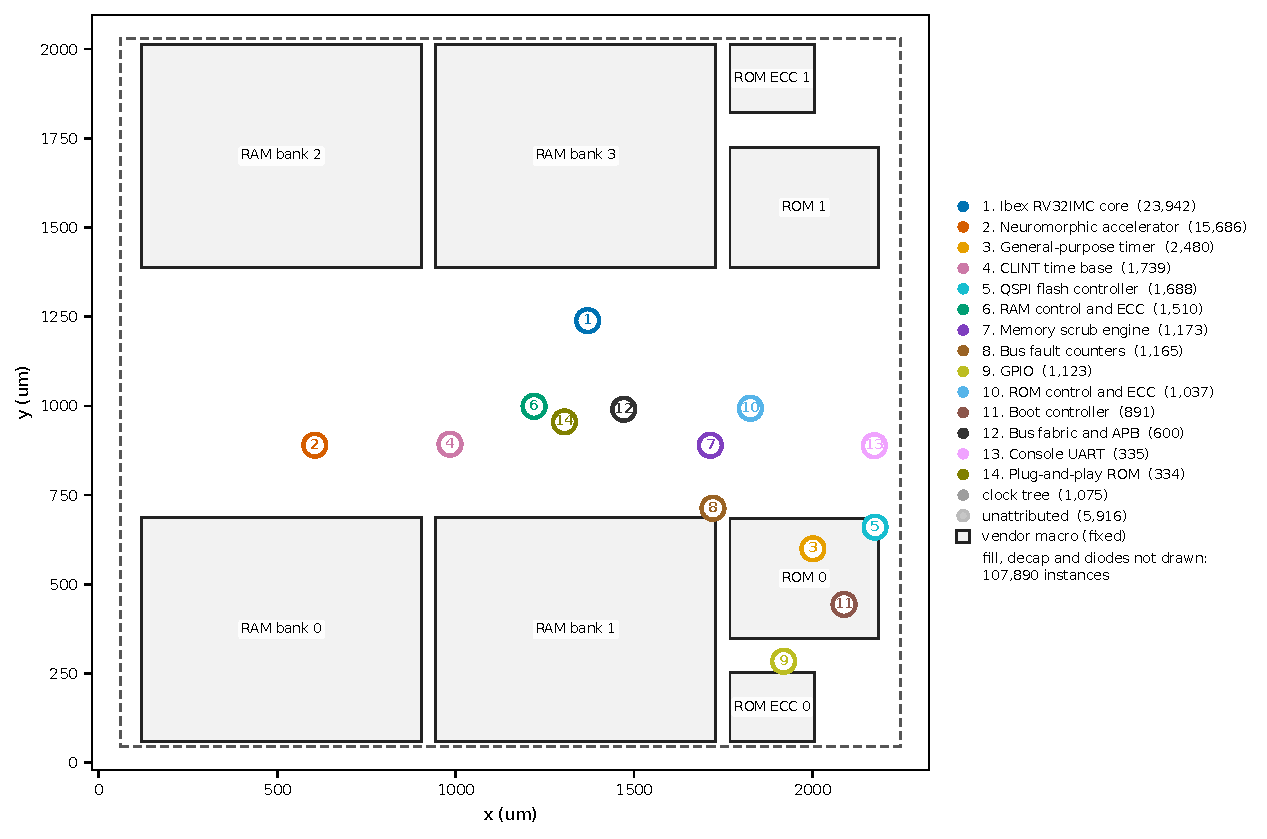
\includegraphics[width=\linewidth]{figures/layout_blocks.pdf}
\caption{Every standard cell of the placed die, coloured by block. Only
about \num{7700} instances still carry a hierarchical name after
synthesis, so attribution is by connectivity --- nets keep their names,
each anonymous cell takes the block most of its pins' nets vote for, and
two rounds of neighbour propagation follow
(\code{thesis/figures/make\_layout\_figures.py}, whose docstring counts
\num{168592} instances where its output file counts \num{168584}; these
figures are the output file's). The remainder, \num{5916} cells or
\SI{9.75}{\percent} of the \num{60694} non-fill cells, is drawn grey
rather than hidden. The protection's own logic is five legend entries
--- RAM control and ECC (\num{1510} cells), the scrub engine
(\num{1173}), the bus fault counters (\num{1165}), ROM control and ECC
(\num{1037}), the boot controller (\num{891}) --- about
\SI{9.5}{\percent} of the non-fill cells [estimate, arithmetic on the
legend].}
\label{fig:harden-blocks}
\end{figure}

\section{Triple modular redundancy, and why one bit cannot have it}
\label{sec:harden-tmr}

Three copies of a flag cannot be held apart. \code{hw/rtl/pilot\_top.v}
section 8.2 proves it: over one bit there are exactly two storage
functions, $x$ and $\lnot x$, so a third replica is bit-for-bit
identical to one of the others and Yosys's \code{opt\_merge} hashes it
away. Over $W$ bits the affine transforms give $2(2^W-1)$ coordinate
functions where three replicas need six, so \textbf{three bits is the
first width at which a third replica has a function left to take}
(\dcite{30}{section 3.3}; \dcite{41}{section 4.1}). Six of the watchdog's eight protected fields
are one bit wide, and replicating one naively yields a single flip-flop
with a voter voting it against itself --- while \textbf{every functional
test and every proof here would still pass}. Polarity cannot rescue it either
(\dcite{33}{section 5}).

So the bits are concatenated into one word and the word is replicated.
Replica A stores $v[i]$, weight 1; B and C store
$\mathrm{enc}_i(v) \oplus \mathrm{POL}[i]$, weight two or three, with
$\mathrm{POL_B} = \lnot\,\mathrm{POL_C}$ --- separated from A because no
function of weight two or more equals $v[i]$ or $\lnot v[i]$, and from
each other by the masks (\dcite{41}{sections 4.2 and 4.3}). The voter is
\code{hw/rtl/tmr\_voter.v}, read in place and never copied, so the SoC's
majority gate is the one \code{formal/tmr\_voter.sby} proves
exhaustively.

\textbf{The bank has no write enable, and that is the scrub.}
Everything in the watchdog is in the power-on reset domain by
requirement W4, so ``written once'' means for the mission, and a bank
that held its value would mask the first upset and then wait for a
second it could not correct. The whole word is therefore written from
the voted value on every clock edge: \textbf{the voter is a continuous
scrubber, and exposure to a second independent upset is one clock cycle
rather than the rest of the mission} (\dcite{41}{section 5.1}). That
bounds accumulation over \emph{time} and nothing else: the header
carries a dated correction saying so, because \dcite{79}{section 1}
measured replicas of this shape sharing rows and abutting.

The watchdog protects eight fields, 22 bits, later 29 when \dcite{43}
added a windowed mode and a kick budget. Worst is \code{dis\_q}, the
bootstrap latch whose corruption sets \code{armed} low so the block
stops for ever; then \code{nmi\_pend}, whose loss means stage 1 never
becomes stage 2, so the watchdog warns for ever without acting
(\dcite{41}{section 3.2}). The report fields are \emph{inside} the
word, because \dcite{16}{section 5.8} had measured this repository's own
safety-net report being the single point of failure: an upset could
erase the announcement of the event it caused.

The ladder the word governs escalates in three stages
(\code{hw/soc/rtl/soc\_wdog.v}, W3): a non-maskable interrupt with one
full timeout for software to notice; then, on a second expiry with the
first unacknowledged, \code{rst\_req\_o} for \code{RST\_CYCLES}, which
the core cannot prevent; then, after \code{ESCALATE} resets since
power-on, an external pin latched until power-on reset, because
resetting has demonstrably not worked and the decision belongs outside
the chip.

The identical bank protects three structures: the watchdog's word at 29
bits, the boot block's at 23 (\dcite{69}), the accelerator connection's
cause bank at 25 (\dcite{55}, widened by \dcite{56}).
\dcite{75}{section 3.3} re-measured all nine replicas by the voter's
fan-in cone, in the block synthesis and in \textbf{every one of the 65
whole-SoC netlists the working tree has kept}, and found $29/29/29$,
$23/23/23$ and $25/25/25$, every set of three disjoint.

\section{The register file}
\label{sec:harden-regfile}

The core's campaign ranked its structures by what their corruption costs
and the answer was unambiguous: the register file is 992 of the core's
\num{2198} injectable RTL bits --- \SI{45}{\percent} --- and carries 3.2
of the 4.9 design-weighted percentage points of wrong-or-dead outcome,
more than everything else in the core combined
(\code{hw/soc/rtl/ibex\_regfile\_secded.v} header, citing \dcite{42}).
That file carries upstream's module name and port list and is given to
the build instead of upstream's own, so the Ibex checkout stays a
pristine clone at the pinned commit; the cost, recorded rather than
glossed, is that an upstream port whose \emph{meaning} changes without
its name changing is caught by nothing (\dcite{43}{section 3.2}).

The codec is \code{hw/rtl/secded\_enc.v} and \code{secded\_dec.v}, read
in place and fixed at 72 bits over 64 --- \emph{one} codec on the die,
which is the objection \dcite{38} raised against lockstep's second one.
One codeword per register with the upper 32 data bits tied off gives the
$(40,32)$ shortening; then one check row is identically zero over a
32-bit field, so the optimiser deletes one flip-flop per register, 31 in
all, and what remains is $(39,32)$, \textbf{the minimal SECDED width for
32 data bits}. The netlist census counts 217 check flip-flops and
would fail at 248 (\dcite{43}{section 6.3}).

Correction on read alone leaves the corruption in the flip-flop, and a
register held across a long call keeps it as long as it holds its value
--- \textbf{the second upset in that word is uncorrectable}. So a
pointer walks \code{x1}\dots\code{x31}, decoding and re-encoding one
register per idle cycle; when the core writes, the scrub stalls and the
pointer holds rather than skipping. The period is \textbf{not proved
bounded}: 31 cycles when the core is idle, unbounded in the limit of a
program that writes the file every cycle for ever
(\dcite{43}{section 6.4}).

At first nothing could read the module's correction counters, because
adding an error output is a patch to \code{ibex\_top.sv}. So
\code{opt\_clean} deleted them and the report cost zero area, with a
test asserting that it did --- \emph{a test whose failure would be the
good news} --- and in silicon a corrected upset and no upset were the
same event (\dcite{43}{section 6.5}). \dcite{44} closed that with three
anchored hunks applied to a \emph{generated} copy of
\code{ibex\_top.v}, never committed, routing the line to
\code{soc\_busstat.v}, demonstrated with a load instruction rather than
a hierarchical read: all four of the core campaign's \code{x23}
records end with the golden answer and with software reading
\code{CNT\_RFSEC = 1}.

It does not protect the addresses --- a corrupted \code{raddr} reaches
the wrong register with a perfectly valid codeword --- nor the other
\SI{55}{\percent} of the core, which carries the highest per-bit rates
in the design.

\section{The time base}
\label{sec:harden-mtime}

\code{mtime} was ranked first for protection by three documents and
protected by none, for the same reason each time: an upset in it is
persistent and silent --- it displaces the architectural clock for ever
--- but it cannot disarm anything, so the backstop went first
(\dcite{58}{section 1}).

The answer is not replication, because a counter has structure a general
register does not. \code{mtime} is the 64-bit data field of a $(72,64)$
codeword whose eight check bits are the only added state. Every tick the
stored word is decoded; the corrected value is what increments, what the
comparator sees and what a bus read returns; and \textbf{the check bits
are re-encoded over the value that goes back in, not over the value that
was stored}. That clause is the whole design: encoding over the stored
value builds an ECC counter that silently does nothing, the code
following the corruption into consistency on the next edge
(\dcite{58}{section 3.1}). Since the word is rewritten every clock the
scrub period is one cycle, so there is no scrubber to build and no
accumulation to bound.

Six designs were synthesised against one baseline
(\dcite{58}{section 4}) and two results are negative. \textbf{The
residue-mod-3 detector that \dcite{41}{section 7.4} proposed as the
cheap answer costs \SI{98.694}{\percent} of what the corrector costs and
corrects nothing}: the cost of any check over a 64-bit counter is the
reduction tree that recomputes it, not the shadow register, so the
flip-flop count, 2 against 8, is not where the money is. And
\dcite{41}'s unsynthesised estimate for replicating \code{mtime} and
\code{mtimecmp} --- ``roughly \SI{27000}{\micro\meter\squared} \dots\
256 more flip-flops'' --- measured at
\SI{25792.0740}{\micro\meter\squared} and \emph{exactly} 256 flip-flops,
\SI{4.68}{\percent} high; a good estimate, recorded as one. The code
corrects the same 64 bits for \SI{50.224}{\percent} of the area of
replicating them.

Two decisions follow the same criterion. That 11 of the 64 bits are
architecturally dead over a five-year mission is an argument \emph{for}
covering them, since deadness bounds the fault-free value and not the
faulty one --- truncation saves \SI{1438.1766}{\micro\meter\squared} and
is ``not a protection; a cheaper failure''
(\dcite{58}{section 4.5}). And \code{mtimecmp} gets nothing: software
rewrites it every deadline, and its worst direction is a missed
deadline, the exact failure the watchdog backs up. The cost that is not area: the CLINT's bounded check went from
\SI{6}{\second} to 18\,min 19\,s and its $k$-induction proof from
\SI{2}{\second} to 5\,min 57\,s, because eight XOR reductions of weight
26 over a 64-bit counter is a hard SMT problem in a way a 22-bit voted
word is not (\dcite{58}{section 9.3}).

\section{The memories}
\label{sec:harden-mem}

\SI{72}{\kibi\byte} of RAM and ROM was long the largest storage with
nothing checking a word read out of it. \dcite{58} expected an easy fit,
because the codec is $(72,64)$ and the RAM macro's row is 64 bits.
\textbf{That coincidence is the problem}: a $(72,64)$ codeword is eight
bits \emph{wider} than the row, and a hard macro has no bit-widening.
Six options were costed from the vendor LEF; keeping
\SI{64}{\kibi\byte} needs a seventh macro at
\SI{+491633.62}{\micro\meter\squared} or
\SI{+257608.51}{\micro\meter\squared} \emph{and} a read-modify-write on
every sub-word store, which is a change to the bus protocol rather than
a wrapper (\dcite{67}{section 3}).

What was built puts the check bits in the row and halves the RAM. A
32-bit word is stored as \textbf{four $(16,8)$ byte codewords}, each the
same Hsiao code with 56 data bits tied off, shortening to the minimal
SECDED width for a byte; four of them is exactly 64 bits, so there is no
seventh macro, no die growth and no read-modify-write, a byte write
landing through the macro's own per-bit write mask with its check bits
beside it. \textbf{The RAM is \SI{32}{\kibi\byte}, not
\SI{64}{\kibi\byte}}, a halving the bring-up program does not notice
because it uses \textbf{192 bytes} of static data plus a stack. An
uncorrectable syndrome answers the read with a bus error, so \textbf{the
recovery is a trap, not a wrong word}.

A word the program never touches is rewritten never, so the memories
need a scrubber, and a bus master would have been a re-proof of a fabric
whose arbiter is written for two. This one lives behind the row port: in
an idle cycle it reads a row; in the next,
if the bus is still not asking, it writes back only the lanes the
decoder corrected; if the bus asks, the bus has the port and the result
is dropped. \textbf{Nothing is ever withheld from the bus}, which is
proved, and a lane reported uncorrectable is \emph{never} written back,
since re-encoding a wrong byte would turn a detected double error into a
valid codeword over a wrong value --- two of the suite's eight mutations
being exactly those failures (\dcite{67}{section 4.3}).

The interval ships at 255 idle cycles, walking the 8192-row RAM in about
2.1 million idle cycles [estimate]. The campaign found the bound that
matters and it is not the expected one: at interval 0 the scrubber
repaired 135 of 360 injections against 36 at the shipped setting ---
\emph{and missed what the slower walk caught}, because the pointer had
left the program's low rows within the first hundred cycles and did not
return inside the run. \textbf{A scrubber's coverage of a row is the
interval between two visits to it}, which is why the interval is a
register (\dcite{67}{section 7.3}).

Placed on the same die the codec costs \SI{+3.01}{\percent} of
standard-cell area, with the die not one database unit larger and hold
closed at three corners. The timing is the honest half. Pre-layout the decoder fit on the read return with
\SI{+2.0352}{\nano\second} of slack; \textbf{post-layout it does not,
and that margin is what layout spent}. The routed path from a macro's
\code{A\_DOUT} to its capturing flip-flop grows from
\SI{12.7286}{\nano\second} to \SI{14.0728}{\nano\second}, and that
group's violating population from \textbf{68 endpoints to \num{1080}}.
Its endpoint is inside the register file: a load's data now crosses the
memory decoder \emph{and} the register file's own SECDED encoder in one
cycle --- \textbf{two independent codes over one word}, which this
project would not have chosen deliberately, and which is still not the
binding path (\dcite{67}{section 5.3}).

\section{Boot}
\label{sec:harden-boot}

Protecting a memory creates a problem at power-on. An SRAM powers up
undefined and \textbf{so does its check field}, so a word nothing has
written is 32 random data bits beside 32 random check bits, and the
codec's answer is an uncorrectable, answered with a bus error
(\dcite{68}{section 4.1}).

\code{boot\_crt0.S} sweeps the whole RAM before the stack pointer is
set, because the loader's own stack, \code{.data} and \code{.bss} are
inside what it is initialising. And it writes \textbf{whole words}: a
byte store makes one of a row's four codewords valid and leaves three as
the SRAM powered up, so ``initialise the RAM'' is not the requirement
--- ``write whole codewords'' is. Both counterfactuals time out at
\num{900095} cycles with a double fault: the loader faults on the first
RAM word nobody wrote, and \emph{the trap handler reads a word nobody
wrote too}. The byte sweep is the instructive one,
leaving \num{1648} uncorrectable rows against no sweep's \num{1706}
while looking initialised (\dcite{68}{section 4.4}). The sweep costs
\num{49178} cycles, \textbf{6.003 per word}, \SI{26.5}{\percent} of the
boot; the image checksum is then computed \emph{from the RAM} rather
than the flash, so a word that arrived intact and landed on a row whose
codeword did not take is caught.

The boot block is 92 flip-flops and \dcite{69} protects \textbf{eighteen}
--- the boot counter, the sampled straps, the watchdog-pin readback, two
validity bits, the sampling delay, and one the campaign added. That one
is the finding. \code{sys\_q} was ranked unprotected because it is
rewritten from \code{rst\_ni} every clock --- true of the register,
false of the consequence, since an upset there manufactures a release
edge, the boot counter increments, and \textbf{the counter is saturating
and power-on-only, so nothing ever takes it back}. Three of four draws
came back as silent corruption and one put the part past its attempt
limit for the power cycle, so it moved into the protected word at a cost
of two flip-flops (\dcite{69}{section 8.4}).

\section{Stopping the clock without losing the report}
\label{sec:harden-clock}

Power, not frequency, is the requirement this design is written against:
\dcite{57} measured \SI{33.890}{\milli\watt} computing and
\SI{5.539}{\milli\watt} waiting at the typical corner, against a
\SI{34.835}{\milli\watt} sign-off figure taken with no switching
activity. \dcite{76} then added two clock gates, and the interesting
part is what gating a fault-tolerant block gets wrong by default. \textbf{A
clock-gated flip-flop still holds state and can still be upset; what it
cannot do is report the upset}, because the voter's correction, the
queue's parity discard and the cause bank's mismatch are all recorded by
registers that need a clock. A sleeping accelerator would have absorbed
the upset and told nobody --- the defect \dcite{52}{section 10} named
and \dcite{55} closed. So all eleven fault lines are terms of the
accelerator's clock-gate enable: \textbf{an upset inside a sleeping
block wakes it up}, at zero cycles of latency, because the enable is
combinational and an integrated clock gate latches it on the falling
edge (\dcite{76}{section 3.2}).

The negative result is that neither clock-gating check closes at the
slow corner --- \SI{-0.7495}{\nano\second} for the fabric's gate and
\SI{-5.0198}{\nano\second} for the accelerator's --- and a violated
setup check at a clock gate is a possible glitch on a clock net, a width
this project has no instrument to measure. \dcite{76} blamed the eleven
fault lines and ranked their removal first; \dcite{77} cut the launch
domains one at a time on that netlist and found the worst path starting
\emph{inside} the accelerator, where every fault line starts, at only
\SI{-1.3129}{\nano\second}, the \SI{-5.0198}{\nano\second} launching
instead from \textbf{the register-file read address that gives the whole
design its worst slack}. The repair was built anyway, for a better
reason: the enable is split by \emph{arrival}, and a term that is a
function of registers the clock has stopped cannot pulse and vanish, so
the cost is \textbf{one cycle of wake latency on a fault and one
flip-flop}, proved rather than hoped (\dcite{77}{sections 1, 3 and 6}).

\section{W9: a correction that cost a reset}
\label{sec:harden-w9}

The sharpest result in the corpus came from measuring the netlist
instead of the RTL. In a gate-level campaign on the watchdog's three
replica banks, \textbf{174 of 174 injected upsets classified CORRECTED
--- and every one of them reset the SoC one clock later}
(\dcite{74}{section 10.2}).

The mechanism is a decode. \code{rst\_req\_o} was
\code{(rst\_hold != 0)}, a five-input OR-reduce of bits 21:17 of the
\emph{voted} word, and two of the three replica outputs are
\code{mix\_dec} of their stored bits --- an XOR tree over all 29
flip-flops of the bank. \code{soc\_top.v} then built
\code{rst\_raw\_n = rst\_ni \&\& !wdog\_rst\_req} and hung the SoC's
reset synchroniser off it \emph{asynchronously}, under a comment reading
``rst\_req is a registered signal in this clock domain''. It was not.
\textbf{The consumer documented the assumption and the producer did not
meet it}, and nothing checked it (\dcite{75}{section 5.1}).

That this is a hazard rather than an intended decode needed no
simulation. Grouping every flip-flop's reset net by the set of
flip-flops feeding it combinationally, the signed-off netlist has
\textbf{five distinct asynchronous-reset source sets}: four are a port
or one or two \emph{registered} signals, and a flip-flop's output does
not glitch. The fifth is \code{rst\_raw\_n}, whose combinational fan-in
is \textbf{25 flip-flops of the three replica banks and nothing else}
(\dcite{75}{section 6}).

The fix is one flip-flop. \code{in\_reset\_q} is the same predicate
computed from the \emph{pre-storage} word rather than the decode, so the
two are equal on every cycle --- proved by $k$-induction as W9a --- and
\code{rst\_req\_o = in\_reset \&\& in\_reset\_q}. The masking is
logical rather than structural, so the mapper may factor it freely; that
it survived mapping is proved by SAT on the mapped cells, with two
mutations that make the proof fail, one of which keeps the flip-flop and
the cell count and gets the logic wrong (\dcite{75}{section 7.4}). It
cost \textbf{one flip-flop} and \SI{+643.0536}{\micro\meter\squared} on
the whole SoC, with no die area, no hold margin at any corner and no
DRC; a block-level area figure was published and then
\textbf{withdrawn} on 2026-09-09 because it did not reproduce under any
of nine recipes, and it is not quoted here.

\begin{table}[tbp]
\centering
\small
\caption{Resets per corrected upset: 174 injections into the same 87
bits at the same 174 cycles, on four netlists mapped on four separate
occasions (\dcite{75}{section 8.5}). The row is the design and the
column is nothing. In all four the vote behaved identically: 174
\textsc{corrected}, one mismatch cycle each, and even \emph{which}
twenty replicas held their corrupted value rather than being rewritten
--- 4, 8 and 8 by bank --- are the same.}
\label{tab:w9}
\begin{tabular}{lcc}
\toprule
 & unrepaired & repaired \\
\midrule
placed and routed layout & $174/174 = 1.0000$ & $0/174 = 0.0000$ \\
synthesis netlist & $174/174 = 1.0000$ & $0/174 = 0.0000$ \\
\bottomrule
\end{tabular}
\end{table}

\section{The evidence}
\label{sec:harden-evidence}

Every campaign classifies each injection into exactly one of five
classes, decided in this order (\dcite{16}{section 1.6}):
\textsc{hang}, the run did not complete inside its cycle budget
\emph{and} nothing was flagged; \textsc{detected}, a design fault flag
or counter moved; \textsc{sdc}, the output differs from the golden model
and nothing was flagged; \textsc{corrected}, the output matches the
golden model \emph{and} a correction counter moved; \textsc{masked}, the
output matches and nothing moved. \textbf{The golden model decides right
from wrong, always}; the design's own flags only decide whether a wrong
answer was announced.

\textsc{corrected}, rather than ``never \textsc{sdc}'', is therefore the
acceptance criterion for a protected bank, because \textbf{an injection
that never reached a flip-flop comes back \textsc{masked}, and
\textsc{masked} is exactly the quiet nothing a mis-targeted injector
produces} (\dcite{41}{section 8.2}). But it cannot be copied: the
register file's campaign demanded it of every injection and failed at
104 of 124 \emph{on a design that was right}, because a register the
program overwrites before the scrub reaches it has shed the upset
without the codec seeing it. The criterion there is now that nothing is
\textsc{sdc} or \textsc{detected} and every \textsc{masked} record is
\emph{explained} (\dcite{43}{section 9.2}).

\begin{table}[tbp]
\centering\footnotesize
\caption{Fault-injection campaigns bearing on the hardening, with their
paired counterfactuals. Every injection is a single-bit flip into one
flip-flop at a seeded-random cycle inside a measured window.}
\label{tab:campaigns}
\begin{tabularx}{\linewidth}{@{}lr>{\raggedright\arraybackslash}X@{}}
\toprule
Population (source) & $n$ & Result \\
\midrule
Watchdog's own state, RTL (\dcite{41}{\,8.2})
 & 162
 & 126 of 126 into the protected word \textsc{corrected}; 0 SDC, 0 HANG,
   0 disarmed. Later 220 draws at 29 bits: 168 of 168 \\
\quad counterfactual, \code{HARDEN = 0}
 & 32
 & 27 SDC, 1 HANG, \textbf{2 left the watchdog reading disarmed}, 6 of
   32 preserved the escalation order \\
Ibex core, campaign A (\dcite{43}{\,8.2})
 & \num{1400}
 & Register-file strata 0 SDC and 0 HANG in 200, against 3 and 4 before;
   0 uncorrectable syndromes. Design-weighted SDC \SI{2.8}{\percent}
   $\pm$ 1.6 $\to$ \SI{1.3}{\percent} $\pm$ 0.4; HANG
   \SI{2.1}{\percent} $\to$ \SI{0.3}{\percent} \\
Ibex core, campaign AW (\dcite{43}{\,8.4})
 & \num{1400}
 & The window rejected a kick as early on 11 draws, 0 on dead machines,
   and produced \textbf{7 spurious escalations in \num{1232} survivable
   upsets} \\
Supervisor workload (\dcite{46}{\,8})
 & 812
 & 32 of 32 dead machines caught, all by ordinary expiry; the window
   converted 2 silent corruptions into announced failures and caused 2
   of 4 spurious escalations \\
Register file alone (\dcite{43}{\,9.2})
 & 124
 & 107 \textsc{corrected}, 17 \textsc{masked}, 0 unexplained. Without
   the scrub: 99 / 25, of which \textbf{6 unexplained} --- upsets still
   sitting in storage nothing had seen \\
CLINT, hardened (\dcite{58}{\,8.3})
 & 342
 & \code{mtime} 128 of 128 and \code{mtime\_chk} 16 of 16
   \textsc{corrected}; clock displaced 0 times; all 144 announced \\
\quad counterfactual, \code{HARDEN = 0}
 & 326
 & 95 of 128 displaced the clock, worst \num{9223372036854775808} ticks
   --- \num{5845} years at \SI{20}{\nano\second} --- and \textbf{0
   announced} \\
Memories, two builds (\dcite{67}{\,7.2--7.3})
 & 720
 & \textbf{0 SDC, 0 traps, 0 hangs}; 104 corrected at the shipped scrub
   interval (68 on a read, 36 by the scrubber), 168 at interval 0 \\
\quad counterfactual, no check bits
 & 280
 & 17 silent wrong answers, 17 announced failures, 1 hang; \textbf{15 of
   the 17 from one constant} the program reads every round \\
Boot block (\dcite{69}{\,8.3})
 & 572
 & 276 of 276 into the protected word \textsc{corrected}; 0 SDC, 0
   spurious give-up, 0 misreported strap \\
\quad counterfactual, \code{HARDEN = 0}
 & 368
 & 261 SDC; 38 corrupted the boot counter, \textbf{worst by 128 boots};
   11 put the part past its attempt limit, 8 stopped it reaching one \\
NPU connection (\dcite{52}{\,1})
 & 700
 & \SI{4.2}{\percent} $\pm$ 1.6 design-weighted silent corruption; 7 of
   600 killed the machine, and the watchdog caught 7 of 7 \\
Core at gate level (\dcite{74}{\,1})
 & \num{1424}
 & \num{1158} of \num{1175} comparable records classify identically to
   RTL; the register file corrected 171 of 180 \emph{in the gates} \\
Watchdog banks, gate level (\dcite{75}{\,8})
 & 174
 & 174 \textsc{corrected} on each of four netlists --- and
   \cref{tab:w9} \\
\bottomrule
\end{tabularx}
\end{table}

Three entries in \cref{tab:campaigns} are negative results, published as
such. The windowed watchdog was built on a recommendation, proved,
measured, and \textbf{its measured value on the first workload was
zero}: 0 of 30 dead machines caught, 0 of 4 on the records replayed
verbatim, seven spurious escalations bought. The recommendation was
aimed at the wrong failure --- a window fires on a kick that is too
\emph{early}, and the runaway that motivated it was a machine executing
its own instructions in order and petting the watchdog on schedule
(\dcite{43}{section 5.1}). What catches that class is a per-phase kick
budget, 4 of 4 on the same records, and the register file removes the
class at source. On a second workload the window's benefit
(\SI{0.25}{\percent}) and cost (\SI{0.27}{\percent}) are the same size,
and \dcite{46}{section 9} recommends removing it before floorplanning
--- which has not been done, the protected word still being 29 bits in
every netlist censused.

It also costs software a rule rather than hardware area, bounding the
jitter ratio of the program's kick cadence: the original workload
measures \textbf{57.2}, which fits inside no window at all, and the
supervisor written to be what the software will be measures 1.412
time-triggered and 2.104 work-triggered --- \textbf{at which no timeout
at all satisfies both bounds} (\dcite{46}{sections 5 and 7}).

\section{TMR blindness}
\label{sec:harden-blind}

A synthesiser is built to delete deliberately redundant logic, and this
project has been burned by exactly that: \code{pilot\_top.v} section 9
records the configuration TMR merging away entirely, and \dcite{38}
measured \SI{15455}{\micro\meter\squared} of an unguarded lockstep the
mapper was removing. The project's own paper states the general form: a
redundancy claim ``was checked at three levels and was wrong at two of
them''. At the register-transfer level it was true; in the mapped
netlist it was false, structural hashing having collapsed three declared
replicas into one physical bank --- \textbf{and the RTL fault-injection
campaign built to detect exactly that produced bit-identical output on
the defective and the repaired design}, because it deposits into signals
the netlist no longer contains (\code{paper/main.tex}, abstract).

Every functional test here would pass on a netlist with one replica
instead of three, and so would every proof: of five mutations against
the composition proof, the last is the honest negative --- turning the
anti-merge transform off keeps \emph{every} property true, because one
bank answering three times still satisfies them
(\dcite{41}{section 9.4}). \textbf{The only honest place to count
replicas is the netlist.} The census in
\code{sw/tests/test\_soc\_synthesis\_guards.py} is built to be able to
fail: with \code{keep} and \code{keep\_hierarchy} deleted from the
\emph{text} of a scratch copy and the flatten forced, the count does not
move --- 102 then, 132 with the wider word and W9, on two independent
technology mappers --- and the mutations it does fail on are invisible
to everything else, \code{.MIX(0)} on replica C costing 11 flip-flops
and on B and C 22 while being functionally identical RTL, bit for bit at
every port (\dcite{41}{sections 6.2 and 6.3}).

Counting is necessary and not sufficient, and \dcite{75} found out how.
Three instruments answer ``which flip-flops belong to this replica'' and
they disagree. By \textbf{instance path} --- what every guard uses ---
the watchdog's banks are $29/29/29$. By \textbf{Q-net name} they are
$29/14/15$, because the polarity masks make exactly one of B and C reset
to one on every bit, the library has no set flip-flop, \code{dfflibmap}
legalises it as a reset-to-zero flop behind an inverter, and \emph{the
resulting cell is not the cell the name was attached to}. By the voter's
\textbf{fan-in cone} they are $29/29/29$ again. A name is a hypothesis.

And a count of the right size can be a count of the wrong thing.
Changing one argument so the voter reads replica A twice produces a
design that passes \emph{every} check in the repository --- per replica,
total, attribute-free, both mappers, every test, every proof --- and
whose vote is a majority over two distinct values, so an upset in
replica A is not masked at all. The union of the three cones falls from
87 to 58; \textbf{the cone census catches it and nothing else does}, and only if
it anchors on the voter's own input pin rather than the bank's output
wire, which still exists in the mutant (\dcite{75}{section 4.3}). Two
rungs followed: a guard running the cone census over every whole-SoC
netlist the tree has kept, since nothing had ever censused the netlist
the foundry would receive; and \code{formal/eqy/}, which checks that the
netlist computes the RTL's \emph{function} for \code{tmr\_voter} --- the
module a flip-flop census structurally cannot check, having no
flip-flops --- with two negative controls whose passing the Makefile
treats as an error (\dcite{79}{section 2}).

The last rung is the die, and there the claim does not survive intact.
On the frozen pilot's sign-off layout the banks are not
placement-separated: minimum cross-replica separation is
\SI{3.78}{\micro\meter} centre-to-centre, the floor for two cells in
adjacent rows, and 49 pairs abut. Against a null model shuffling only
the replica labels over the same placed positions the banks are
indistinguishable from an arbitrary labelling --- $110.73 \pm 8.26$
expected, 103 observed --- so the finding is not that the placer drew
them together but that \textbf{it did not keep them apart}. What is
measured as a mechanism is a \textbf{4.12-fold concentration on
corresponding bits}: median \SI{27.52}{\micro\meter} against
\SI{113.47}{\micro\meter} over all cross-replica pairs, the shape a
shared voter's wirelength would leave. The same picture appears on
\code{soc\_top} across all three of its TMR structures and two
independent hardens (\dcite{79}{sections 1.2--1.6}).

The limit is carried here unchanged from \dcite{79}{section 3}.
\textbf{A distance is not a safety argument in either direction.} No
single-event cross-section or LET threshold for this process was
measured and none is available; the measurement establishes that this
layout \emph{permits} a common-mode upset over much of the protected
word and says nothing about whether one occurs at any fluence.
``Because the replicas are a few micrometres apart, one ion track
defeats the vote'' is therefore forbidden: it silently supplies a
conversion this work does not have. What it does change is the prose ---
every unqualified sentence saying the configuration is protected by
triple modular redundancy must read \emph{triplicated in the netlist}.
The measurement does not make those sentences false; it removes their
evidence. No placement constraint was applied, and the one time
placement was constrained here the region form did not route and the
manual form cost about \SI{7}{\nano\second} of worst slack.

\section{What it costs}
\label{sec:harden-cost}

\begin{table}[tbp]
\centering\footnotesize
\caption{Measured area of each mechanism, against a baseline measured in
the same session with only the thing being priced turned off. Gate
equivalent is \code{sg13g2\_nand2\_1} $=$
\SI{7.2576}{\micro\meter\squared}; the Ibex reference is
\SI{275682.6198}{\micro\meter\squared}. Deltas are arithmetic on two
measurements [estimate]; every measured row is [fact]. Rows marked
$\dagger$ are deltas on the whole SoC rather than on one block.}
\label{tab:harden-area}
\begin{tabular}{@{}lrrr@{}}
\toprule
Mechanism & $\Delta$ flops & $\Delta$ area (\si{\micro\meter\squared}) & of Ibex \\
\midrule
Watchdog TMR, W6 (\dcite{41}{\,6.5}) & $+49$ & $+5{,}091.0552$ & $+1.85\,\%$ \\
Windowed mode and kick budget (\dcite{43}{\,7.3}) & $+29$ & $+4{,}904.0964$ & $+1.78\,\%$ \\
SECDED register file (\dcite{43}{\,7.1}) & $+222$ & $+38{,}050.5762$ & $+13.80\,\%$ \\
\quad of which the scrub, module alone (\dcite{43}{\,7.2}) & $+5$ & $+9{,}963.5130$ & --- \\
\code{mtime} SECDED, H6 (\dcite{58}{\,7}) & $+8$ & $+7{,}026.8310$ & $+2.549\,\%$ \\
\quad its report in BUSSTAT & $+18$ & $+1{,}917.4050$ & $+0.695\,\%$ \\
Boot decision word, B1 (\dcite{69}{\,1}) & $+51$ & $+5{,}255.9010$ & $+1.9065\,\%$ \\
Memory ECC and scrub engine$^{\dagger}$ (\dcite{67}{\,5.1}) & $+234$ & $+31{,}391.3124$ & --- \\
W9, registered reset request$^{\dagger}$ (\dcite{75}{\,1}) & $+1$ & $+643.0536$ & --- \\
Registered clock-gate wake$^{\dagger}$ (\dcite{77}{\,1}) & $+1$ & $+829.4454$ & --- \\
\midrule
\emph{Declined:} lockstep, for \emph{detection} (\dcite{38}{\,8.5}) & --- & $+309{,}550$ & $+112\,\%$ \\
\emph{Declined:} TMR over \code{mtime}, \code{mtimecmp} (\dcite{58}{\,4}) & $+256$ & $+25{,}792.0740$ & $+9.356\,\%$ \\
\emph{Declined:} residue-mod-3 detector (\dcite{58}{\,4}) & $+2$ & $+6{,}935.0904$ & --- \\
\bottomrule
\end{tabular}
\end{table}

Two habits sit behind \cref{tab:harden-area}, both learned by nearly
getting a number wrong. \textbf{The baseline must be the same source
measured now, with only the priced thing turned off}, never a figure a
previous document published: three waves measured that gap at
\SI{58.17}{\micro\meter\squared}, \SI{25.4394}{\micro\meter\squared}
and \SI{10.9242}{\micro\meter\squared}, the last in the direction that
would have \emph{over}stated the hardening (\dcite{41}{section 6.5};
\dcite{58}{section 7}; \dcite{69}{section 7.1}). And \textbf{a module
measured alone understates what it costs in place}: the register file's
standalone delta is \SI{+31709.55}{\micro\meter\squared} against a
whole-core \SI{+38050.58}{\micro\meter\squared}, \SI{20}{\percent}
larger, because \code{abc} re-optimises across a boundary the flattened
core does not have (\dcite{43}{section 7.2}).

\begin{table}[tbp]
\centering\footnotesize
\caption{Costs that are not area.}
\label{tab:harden-cycles}
\begin{tabularx}{\linewidth}{@{}l>{\raggedright\arraybackslash}X@{}}
\toprule
What & Cost \\
\midrule
Every RTL hardening wave
 & \textbf{Zero cycles.} The whole-SoC self-test reproduced to the cycle
   across each wave: \num{185443} cycles
   (\code{docs/40}--\code{docs/44}), \num{215428}
   (\code{docs/55}--\code{docs/58}), \num{217682}
   (\code{docs/66}--\code{docs/67}), \num{220256} for the program with
   \num{415324} for the run since the boot flow (\dcite{68}{\,8},
   reproduced by \dcite{75}{\,7.5} and \dcite{77}{\,7}). In a fault-free
   machine every decoder is the identity, proved by induction; the
   invariant moves when the program or design gains content, never when
   a protection is added \\
Register-file scrub
 & 31 cycles per sweep when the core is idle; stalls on any cycle the
   core writes; \textbf{period not proved bounded} (\dcite{43}{\,6.4}) \\
\code{mtime} scrub & 1 cycle, by construction (\dcite{58}{\,3.2}) \\
Memory scrub
 & One walk of \num{8192} rows per \num{2100000} idle cycles at the
   shipped interval of 255 [estimate] (\dcite{67}{\,4.3}) \\
Boot RAM sweep
 & \num{49178} cycles, 6.003 per word --- \SI{26.5}{\percent} of the
   boot --- plus 17.01 cycles per word to verify the image out of the
   RAM (\dcite{68}{\,4.2}) \\
Windowed watchdog
 & A bound on the software's kick-jitter ratio,
   $i_{\max}/i_{\min} < 1/(1-2^{-\mathrm{WINS}})$, paid by the program
   (\dcite{43}{\,4.2}) \\
Clock-gate wake
 & Zero cycles as first built; \textbf{one cycle on a fault} after the
   enable was split by arrival (\dcite{77}{\,1}) \\
Register-file read path
 & \SI{2.7928}{\nano\second} at the slow corner, on the module where
   nothing else can move; \SI{0.2593}{\nano\second} recovered for
   \SI{+1201.5486}{\micro\meter\squared} (\dcite{44}{\,5.4}) \\
Memory read return
 & \SI{+1.3442}{\nano\second} routed, that group's violating population
   from 68 endpoints to \num{1080} (\dcite{67}{\,5.3}) \\
Formal
 & The CLINT's bounded check \SI{6}{\second} $\to$ 18\,min 19\,s, its
   proof \SI{2}{\second} $\to$ 5\,min 57\,s (\dcite{58}{\,9.3}) \\
\bottomrule
\end{tabularx}
\end{table}

One line of \cref{tab:harden-cycles} deserves its own sentence, because
the first version of it was wrong. \dcite{43}{section 7.4} attributed a
setup-slack loss and a closure period moving from
\SI{15.98}{\nano\second} to \SI{17.62}{\nano\second} to the register
file's decoder, reasoning that the decoder sits on the read path and the
read path feeds the ALU. \dcite{44} looked at the paths. \textbf{All ten
worst setup paths at the slow corner, in both configurations, start at
\code{cheriot\_enable\_i[0]} --- a configuration input \code{soc\_top.v}
drives with a constant}, which a register-file decoder cannot be on. And
the binding check in the hardened build is not a logic path at all: it
is the \emph{asynchronous reset recovery check} on an unbuffered
\num{2328}-fanout net, with the two hardened builds reporting
bit-identical slacks at every probe. What the protection cost there is
222 more flip-flops on an unbuffered reset net, a place-and-route
obligation and not a logic cost. \textbf{The delta was real and the
attribution was not} (\dcite{44}{sections 5.1 and 5.3}). Consistently
with \dcite{53}{section 9.2} and \dcite{05}{section 4} rule 5,
\emph{no clock frequency is claimed for this design anywhere}; slack
against a \SI{20}{\nano\second} SDC period, with its corner named, is
what is reported.

\section{Four shapes an error takes here}
\label{sec:harden-shapes}

The project keeps a catalogue of the mistakes it makes, because the
shapes repeat and the catalogue is worth more than any single number in
it (\dcite{64}{section 3}; \code{ROADMAP.md} section 3). Four bear on
hardening. They are findings, not apologies.

\paragraph{A green result read wider than what it looked at.}
\dcite{41}{section 6.6} lists eight instances by document and section,
\dcite{43}{section 10} makes it ten, \dcite{58}{section 11} eleven. The
canonical case is the netlist census: it counts flip-flops and asserts
nothing about any other cell, nothing about placement, and nothing about
whether the replicas are \emph{correct}. The fix is never to widen the
claim; it is to build a second instrument at the level the
first cannot see, with a mutation that makes it fail --- which is why
the cone census, the shipped-netlist guard, the equivalence check and
the gate-level campaign all exist. One instance is the shape at its
purest: a mutation harness reported a pass because a build failure
produced no \code{FAIL} lines to parse.

\paragraph{A measured delta attributed to the wrong cause.}
The register file's timing cost is the clearest case: the number moved,
the explanation was wrong, and only looking at the paths found it. The
clock-gate diagnosis of section~\ref{sec:harden-clock} is a second, and
\dcite{61}'s \SI{+4.4}{\percent} estimate --- an earlier absolute area
carried onto a new denominator, measured at \SI{+4.9406}{\percent} by
\dcite{62}{section 1} --- is a third, where the method was the error
rather than the arithmetic. The defence is an
instrument's own resolution: \dcite{44}{section 5.2} measured this
flow's noise floor at about \SI{0.4}{\nano\second} at synthesis, and
\dcite{70} measured it after layout with a control pair that changes
nothing a designer would call a change --- it moves hold by
\SI{0.0198}{\nano\second} and setup by \SI{0.5031}{\nano\second}.

\paragraph{One change leaking in from several places.}
A delta is only a delta if the two runs were asked the same question,
and the answer is a paired counterfactual on identical draws.
\dcite{55}{section 8.3} had to refuse a \SI{19}{\percent} improvement
because its control stratum moved on 15 of 100 records; \dcite{58}
reports its delta because a field-by-field diff over the strata it does
not touch found \textbf{0 of 198 records changed}, and \dcite{69} found
the same zero over 296. \dcite{44} re-ran the entire core campaign and found the two
\num{1400}-record files \emph{byte-identical}, which is stronger than
``the rates agree'', since two records moving in opposite directions
would satisfy that too. The same discipline forced the isolation builds
of \dcite{43}{section 5.4}: with both the window and the budget armed,
both counters have fired by the end of a run that reset itself, and a
report reading them would have credited the window with a catch it did
not make.

\paragraph{The synthesiser deleting redundancy.}
Section~\ref{sec:harden-blind}. The specific hazard is that
\emph{everything else stays green}: the collapsed design satisfies every
property of the composition proof, passes every functional test, and
produces bit-identical fault-injection output. Redundancy is the one
property whose evidence cannot live in the source, because the source is
precisely what the mapper is entitled to rewrite.

\section{What is still open}
\label{sec:harden-open}

\textbf{No radiation data exists for this process.} Neither open PDK
publishes total-ionising-dose or single-event figures, no silicon of
this SoC exists, and no beam time has been taken. Every reliability
number here is a seeded fault-injection measurement on RTL or a placed
netlist, conditional on an upset having landed inside a measured window.
The project has no upset rate $\lambda$ and says so where the arithmetic
would need one (\dcite{67}{section 6.2}).

\textbf{Every campaign is single-bit and flip-flop only}, with no
multi-bit strike and no single-event transient in combinational logic
--- a larger gap for a code than for a replicated bank, because the
code's defence \emph{is} combinational logic, the CLINT's exposed codec
alone being 528 cells (\dcite{58}{section 11}).

\textbf{Addresses are unprotected everywhere}, so a corrupted
register-file address, memory row address or bank select reaches the
wrong location with a perfectly valid codeword, and \textbf{no whole-SoC
campaign reaches a peripheral}. \textbf{The ROM's contents are not
protected in a flight part}: on this PDK the boot ROM is an SRAM that
powers up undefined and nothing in the design can write it, so its check
macros are check bits nobody can initialise; the flight answer is a mask
ROM whose bit is a via and has no stored-upset mechanism
(\dcite{67}{section 8}; \dcite{68}{section 3}). \textbf{And the vendor
macros cannot be signed off on this PDK version}, so neither can the die
that carries them.
